%%%%%%%%%%%%%%%%%%%%%%%%%%%%%%%%%%%%%%%%%
% Wenneker Assignment
% LaTeX Template
% Version 2.0 (12/1/2019)
%
% This template originates from:
% http://www.LaTeXTemplates.com
%
% Authors:
% Vel (vel@LaTeXTemplates.com)
% Frits Wenneker
%
% License:
% CC BY-NC-SA 3.0 (http://creativecommons.org/licenses/by-nc-sa/3.0/)
% 
%%%%%%%%%%%%%%%%%%%%%%%%%%%%%%%%%%%%%%%%%

%----------------------------------------------------------------------------------------
%	PACKAGES AND OTHER DOCUMENT CONFIGURATIONS
%----------------------------------------------------------------------------------------

\documentclass[11pt]{scrartcl} % Font size

%%%%%%%%%%%%%%%%%%%%%%%%%%%%%%%%%%%%%%%%%
% Wenneker Assignment
% Structure Specification File
% Version 2.0 (12/1/2019)
%
% This template originates from:
% http://www.LaTeXTemplates.com
%
% Authors:
% Vel (vel@LaTeXTemplates.com)
% Frits Wenneker
%
% License:
% CC BY-NC-SA 3.0 (http://creativecommons.org/licenses/by-nc-sa/3.0/)
% 
%%%%%%%%%%%%%%%%%%%%%%%%%%%%%%%%%%%%%%%%%

%----------------------------------------------------------------------------------------
%	PACKAGES AND OTHER DOCUMENT CONFIGURATIONS
%----------------------------------------------------------------------------------------

\usepackage{amsmath, amsfonts, amsthm} % Math packages

\usepackage{listings} % Code listings, with syntax highlighting

\usepackage[main = greek, english]{babel} % English language hyphenation

\usepackage{graphicx} % Required for inserting images
\graphicspath{{Figures/}{./}} % Specifies where to look for included images (trailing slash required)

\usepackage{booktabs} % Required for better horizontal rules in tables

\usepackage{dirtytalk} % Required for quoting.

\usepackage{float} % Added for hard placement of images.

\usepackage[dvipsnames]{xcolor} % Added for extra colors.

\usepackage{tikz} % For colored boxes and more.

\numberwithin{equation}{section} % Number equations within sections (i.e. 1.1, 1.2, 2.1, 2.2 instead of 1, 2, 3, 4)
\numberwithin{figure}{section} % Number figures within sections (i.e. 1.1, 1.2, 2.1, 2.2 instead of 1, 2, 3, 4)
\numberwithin{table}{section} % Number tables within sections (i.e. 1.1, 1.2, 2.1, 2.2 instead of 1, 2, 3, 4)

\usepackage{enumitem} % Required for list customisation
\setlist{noitemsep} % No spacing between list items

%----------------------------------------------------------------------------------------
%	DOCUMENT MARGINS
%----------------------------------------------------------------------------------------

\usepackage{geometry} % Required for adjusting page dimensions and margins

\geometry{
	paper=a4paper, % Paper size, change to letterpaper for US letter size
	top=2.5cm, % Top margin
	bottom=3cm, % Bottom margin
	left=3cm, % Left margin
	right=3cm, % Right margin
	headheight=0.75cm, % Header height
	footskip=1.5cm, % Space from the bottom margin to the baseline of the footer
	headsep=0.75cm, % Space from the top margin to the baseline of the header
	%showframe, % Uncomment to show how the type block is set on the page
}

%----------------------------------------------------------------------------------------
%	FONTS
%----------------------------------------------------------------------------------------

\usepackage[utf8]{inputenc} % Required for inputting international characters
\usepackage[T1]{fontenc} % Use 8-bit encoding

%----------------------------------------------------------------------------------------
%	SECTION TITLES
%----------------------------------------------------------------------------------------

\usepackage{sectsty} % Allows customising section commands

\sectionfont{\vspace{6pt}\centering\normalfont\scshape} % \section{} styling
\subsectionfont{\normalfont\bfseries} % \subsection{} styling
\subsubsectionfont{\normalfont\itshape} % \subsubsection{} styling
\paragraphfont{\normalfont\scshape} % \paragraph{} styling

%----------------------------------------------------------------------------------------
%	HEADERS AND FOOTERS
%----------------------------------------------------------------------------------------

\usepackage{scrlayer-scrpage} % Required for customising headers and footers

\ohead*{} % Right header
\ihead*{} % Left header
\chead*{} % Centre header

\ofoot*{} % Right footer
\ifoot*{} % Left footer
\cfoot*{\pagemark} % Centre footer

\newcommand{\img}[1]
{
    \begin{center}
        \fcolorbox{black}{white}{\includegraphics[height=10em]{#1}}
    \end{center}

}

% Helper Macros

\newcommand{\en}[1]{\foreignlanguage{english}{#1}}
\newcommand{\src}[1]{{\ttfamily\en{#1}}}


% Extra Formatting

\setlength{\parindent}{0em}
\setlength{\parskip}{1em}
 % Include the file specifying the document structure and custom commands

\usepackage{subcaption}
\usepackage{amsmath}

\usepackage{pgfplots}
\pgfplotsset{compat = newest}

%----------------------------------------------------------------------------------------
%	TITLE SECTION
%----------------------------------------------------------------------------------------

\title{	
	\normalfont\normalsize
	\textsc{Πανεπιστήμιο Πατρών, Τμήμα Ηλεκτρολόγων Μηχανικών και Τεχνολογίας Υπολογιστών}\\ % Your university, school and/or department name(s)
	\vspace{25pt} % Whitespace
	\rule{\linewidth}{0.5pt}\\ % Thin top horizontal rule
	\vspace{20pt} % Whitespace
	{\Large Εργασία: \en{Pokemon}}\\ % The assignment title
	\vspace{12pt} % Whitespace
	\rule{\linewidth}{2pt}\\ % Thick bottom horizontal rule
	\vspace{12pt} % Whitespace
}

\author{\LARGE Ευάγγελος Λάμπρου \\ \en{UP1066519}} % Your name

\date{} % Today's date (\today) or a custom date

\begin{document}

\maketitle 

\tableofcontents

\newpage

\section{Εισαγωγή}

\section{Ερωτήματα Εργασίας}

\subsection{Μέρος Α}

\subsubsection{Δημιουργία σκηνής κόσμου.}

Ο κόσμος τη εργασίας είναι ένα απλό τοπίο αποτελούμενο από δέντρα και βράχους. Σε κάθε εκτέλεση της εφαρμογής
δημιουργείται ένα νέο τυχαίο τοπίο, με τα αντικείμενα της σκηνής να τοποθετούνται σε τυχαίες θέσεις. 

Για το \en{skybox}, ακολούθησαμε την τεχνική όπου τοποθετούμε στον ορίζοντα το μοντέλο ενός κύβου το οποίο 
στις πλευρές του έχει σαν \en{texture} την κάθε μία από τις όψεις του ουρανού.

% Skybox picture

Δώσαμε ακόμα στον κόσμο έναν κύκλο ημέρας-νύκτας, αλλάζοντα το χρώμα του \en{skybox} σταδιaκά. Συγκεκριμένα, 
εφαρμόζουμε \en{interpolation} \say{ανταλλάζοντας} τα \en{red} και \en{blue} \en{channels} με βάση μία ημιτονοειδή συνάρτηση.

% Two skybox pictures: night and day

\begin{equation}
    color = mix(color_{texture}.bgr, color_{texture}.rgb, \frac{sin(time) + 1}{2})
\end{equation}

\begin{figure}[H]
    \begin{center}
    \begin{tikzpicture}
        \begin{axis}[xmin=0, xmax=10*pi, ymin=-1, ymax=1]
            \addplot[
                domain = 0:10*pi,
                samples = 200,
                smooth,
                thick,
            ] {sin(30*x)};
        \end{axis}
    \end{tikzpicture}
        \caption{Η συνάρτηση ημιτόνου.}
        \end{center}
\end{figure}

Ως πηγή φωτισμού θεωρούμε τον ήλιο. Συνεπώς ερφαρμόζουμε την τεχνική \en{directional lighting} όπου 
κάθε \en{vertex} των αντικειμένων της σκηνής μας φωτίζονται από την ίδια κατεύθυνση ανεξαρτήτως της θέσης τους.
Πρακτικά θεωρούμε πως η πηγή φωτός απέχει μία άπειρη απόσταση από τα υπόλοιπα αντικείμενα της σκηνής μας.
Έτσι, τοποθετήσαμε προσεγγιστικά τον ήλιο σε ένα \say{ψηλό} σημείο. 

% Sun pictures

\subsubsection{Μέθοδος σκίασης}

Η σκίαση της σκηνής αποτέλεσε ένα από τα δυσκολότερα μέρη της εργασίας. Ωστόσο, το τελικό αποτέλεσμα 
είναι ικανοποιητικό. 

Η μέθδος που χρησιμοποιήσαμε είναι αυτή του \en{shadow mapping}. Ζωγραφίζουμε την σκηνή από την πλευρά 
της πηγής φωτός (του ήλιου) σε ένα \en{texture} στο οποίο αποτυπώνεται η απόσταση του κάθε αντικειμένου 
από το φως. Έτσι, μπορούμε να συμπεράνουμε εάν ένα σημείο σκιάζεται. 

Για να δωθεί περαιτέρω η αίσθηση για το πέρασμα του χρόνου, έχουμε την φωτεινή πηγή να κινείται 
γύρω από τη σκηνή για να προσομοιώσει την κίνηση του ήλιου. 
Για αυτό το λόγο στη σκηνή μας περιοριζόμαστε σε \en{dynamic shadows}.

% Picture with shadows

\subsubsection{Περιήγηση στη σκηνή και φυσική αλληλεπίδραση}

Για την περιήγηση του χρήστη στη σκηνή, δημιοργήσαμε μία οντότητα κάμερας η οποία είναι υπεύθυνση 
για τον υπολογισμό των \en{view} και \en{projection} πινάκων με βάση μία δεδομένη θέση και κατεύθυνση όρασης.


\subsection{Μέρος Β}

\subsubsection{Εμφάνιση τέρατος}

\subsubsection{Παγίδευση τέρατος}

\subsubsection{Επίθεση τέρατος}

\subsection{Bonus}

\subsubsection{Εξέλιξη τέρατος}

\begin{figure}[H]
	\begin{center}
		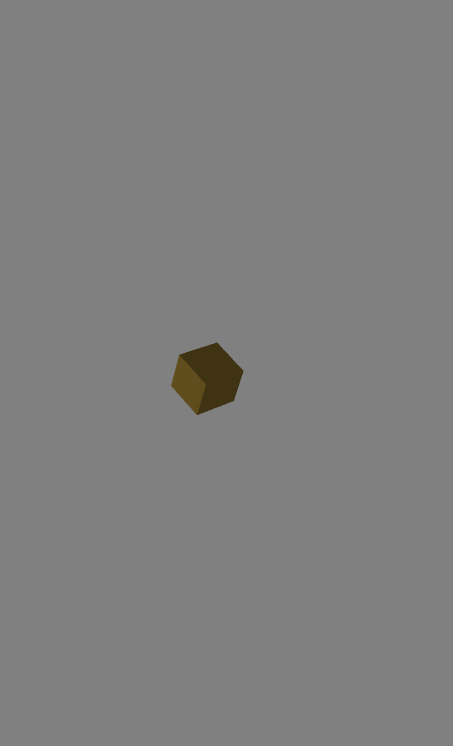
\includegraphics[height=.5\textheight]{./assets/cube.png}
	\end{center}
	\caption{Ο κύβος να περιστρέφεται}
\end{figure}

\end{document}
